\begin{frame}
\begin{center}
\Huge{Numpy and Scipy}
\end{center}
\end{frame}

\begin{frame}
\begin{center}
\Huge{Numpy}
\end{center}
\end{frame}

\begin{frame}[fragile]
    \frametitle{NumPy}
We need to import \verb#numpy# for the following examples:
    \begin{myColorBox}{0.9}{}
\begin{verbatim}
import numpy as np 
\end{verbatim}
    \end{myColorBox}
Numpy arrays:
    \begin{myColorBox}{0.9}{}
\begin{verbatim}
>>> a = np.array( [2, 3, 4] )
>>> a
array([2, 3, 4])
>>> type(a) 
<type 'numpy.ndarray'>
\end{verbatim}
    \end{myColorBox}
    \pause
    \begin{myColorBox}{0.9}{}
\begin{verbatim}
>>> b = np.array( [ (1.5, 2, 3), (4, 5, 6) ] )
>>> b
array([[ 1.5,  2. ,  3. ],
       [ 4. ,  5. ,  6. ]])
\end{verbatim}
    \end{myColorBox}
\end{frame}

\begin{frame}[fragile]
    \frametitle{NumPy}
    \begin{myColorBox}{0.9}{}
\begin{verbatim}
>>> b.ndim     # number of dimensions
2
>>> b.shape    # the dimensions
(2, 3)
>>> b.dtype    # the type (8 byte floats)
dtype('float64')
>>> b.itemsize # the size of the type
8
\end{verbatim}
    \end{myColorBox}
    \pause    
    \begin{myColorBox}{0.9}{}
\begin{verbatim}
>>> c = np.array( [ [1, 2], [3, 4] ], dtype=complex )
>>> c
array([[ 1.+0.j,  2.+0.j],
       [ 3.+0.j,  4.+0.j]])
>>> d = np.array( [ [1+3j, 2], [3+2.5j, 4] ],
				 dtype=complex )
array([[ 1.+3.j ,  2.+0.j ],
       [ 3.+2.5j,  4.+0.j ]])
\end{verbatim}
    \end{myColorBox}
\end{frame}

\begin{frame}[fragile]
\frametitle{NumPy}
You can define your own dtypes. Suppose you have the following array of tuples:
\begin{myColorBox}{1.0}{}
\begin{verbatim}
>>> x = np.array([[('Christian', 43887651), 
('John', 90117628)],
[('Martha', 43887651), 
('Stephen', 90117628)]])
>>> x
array([[['Christian', '43887651'],
        ['John', '90117628']],
       [['Martha', '43887651'],
        ['Stephen', '90117628']]], 
      dtype='|S9')
>>> dt = np.dtype({'names':('name','phone'),
'formats':('|S8', 'i8')})
>>> x = np.array([[('Christian', 43887651), 
('John', 90117628)],
[('Martha', 43887651), 
('Stephen', 90117628)]], dtype=dt)
>>> x
array([[('Christia', 43887651), ('John', 90117628)],
       [('Martha', 43887651), ('Stephen', 90117628)]], 
      dtype=[('name', '|S8'), ('phone', '<i8')])
\end{verbatim}
\end{myColorBox}
\end{frame}

\begin{frame}[fragile]
\frametitle{}
\begin{myColorBox}{1.0}{}
\begin{verbatim}
>>> x['name']
array([['Christia', 'John'],
       ['Martha', 'Stephen']], 
      dtype='|S8')
>>> x[0,0]
('Christia', 43887651)
>>> x['phone'][0,0]
43887651
>>> x[1] = ('Julia',11324455)
>>> x
array([[('Christia', 43887651), ('John', 90117628)],
       [('Julia', 11324455), ('Julia', 11324455)]], 
      dtype=[('name', '|S8'), ('phone', '<i8')])
\end{verbatim}
\end{myColorBox}
\end{frame}

\begin{frame}[fragile]
    \frametitle{NumPy}
A more useful example! Suppose you have a file with entries that look like
this:
\begin{verbatim}
CLC -1.175975e+02 3.581574e+01 soil
SLA -1.172833e+02 3.589095e+01 rock
GRA -1.173662e+02 3.699608e+01 soil
TIN -1.182301e+02 3.705422e+01 soil
\end{verbatim}
    \pause    
    \begin{myColorBox}{1.0}{}
\begin{verbatim}
>>> stdat = np.loadtxt('station_data.txt',
dtype={'names':('stname', 'lon', 'lat', 'substrate'),
'formats': ('|S4', 'f8', 'f8', '|S4')})
>>> stdat
array([('CLC', -117.5975, 35.81574, 'soil'),
       ('SLA', -117.2833, 35.89095, 'rock'),
       ('GRA', -117.3662, 36.99608, 'soil'),
       ('TIN', -118.2301, 37.05422, 'soil')], 
      dtype=[('stname', '|S4'), ('lon', '<f8'),
       ('lat', '<f8'), ('substrate', '|S4')])
>>> stdat['stname']
array(['CLC', 'SLA', 'GRA', 'TIN'], 
      dtype='|S4')
>>> stdat['lon']
>>> array([-117.5975, -117.2833, -117.3662, -118.2301])
\end{verbatim}
    \end{myColorBox}
\end{frame}


\begin{frame}[fragile]
    \frametitle{NumPy}
Create arrays:
    \begin{myColorBox}{1.0}{}
\begin{verbatim}
>>> np.zeros( (3, 4) )  # parameter specify the shape
array([[0.,  0.,  0.,  0.],
       [0.,  0.,  0.,  0.],
       [0.,  0.,  0.,  0.]])
>>> np.ones( (2, 3, 4), dtype=int16 ) # dtype specified
array([[[ 1, 1, 1, 1],
        [ 1, 1, 1, 1],
        [ 1, 1, 1, 1]],
       [[ 1, 1, 1, 1],
        [ 1, 1, 1, 1],
        [ 1, 1, 1, 1]]], dtype=int16)
\end{verbatim}
    \end{myColorBox}
Supported data types: bool, uint8, uint16, uint32, uint64, int8, int16, int32, int64, float32, float64, float96, complex64, complex128, complex192 
\end{frame}

\begin{frame}[fragile]
    \frametitle{NumPy}
    \begin{myColorBox}{1.0}{}
\begin{verbatim}
>>> np.empty( (2,3) )
array([[  3.73603959e-262,   ...,   ...],
       [  5.30498948e-313,   ...,   ...]])
\end{verbatim}
    \end{myColorBox}
    \pause
    \begin{myColorBox}{1.0}{}
\begin{verbatim}
>>> np.arange( 10, 30, 5 )
array([10, 15, 20, 25])
>>> np.arange( 0, 2, 0.3 ) # it accepts float arguments
array([ 0. ,  0.3,  0.6,  0.9,  1.2,  1.5,  1.8])
\end{verbatim}
    \end{myColorBox}
    \pause
    \begin{myColorBox}{1.0}{}
\begin{verbatim}
>>> np.linspace( 0, 2, 9 ) # 9 numbers from 0 to 2
array([ 0.  ,  0.25,  0.5 ,  0.75, ...,  2.  ])
>>> x = np.linspace( 0, 2*pi, 100 )
>>> f = np.sin(x)
\end{verbatim}
    \end{myColorBox}
\end{frame}

\begin{frame}[fragile]
\frametitle{Numpy}
Creating grids
\begin{myColorBox}{0.9}{}
\begin{verbatim}
>>> x = np.arange(0.0,1.1,0.1)
>>> y = x
>>> xx, yy = np.meshgrid(x,y)
>>> xx
array([[ 0. ,  0.1,  0.2, ...,  0.8,  0.9,  1. ],
       [ 0. ,  0.1,  0.2, ...,  0.8,  0.9,  1. ],
       [ 0. ,  0.1,  0.2, ...,  0.8,  0.9,  1. ],
       ..., 
       [ 0. ,  0.1,  0.2, ...,  0.8,  0.9,  1. ],
       [ 0. ,  0.1,  0.2, ...,  0.8,  0.9,  1. ],
       [ 0. ,  0.1,  0.2, ...,  0.8,  0.9,  1. ]])
>>> yy
array([[ 0. ,  0. ,  0. , ...,  0. ,  0. ,  0. ],
       [ 0.1,  0.1,  0.1, ...,  0.1,  0.1,  0.1],
       [ 0.2,  0.2,  0.2, ...,  0.2,  0.2,  0.2],
       ..., 
       [ 0.8,  0.8,  0.8, ...,  0.8,  0.8,  0.8],
       [ 0.9,  0.9,  0.9, ...,  0.9,  0.9,  0.9],
       [ 1. ,  1. ,  1. , ...,  1. ,  1. ,  1. ]])
\end{verbatim}
\end{myColorBox}
\end{frame}

\begin{frame}[fragile]
\frametitle{}
\begin{myColorBox}{0.9}{}
\begin{verbatim}
>>> plt.contourf(xx,yy,
np.sin(xx*np.pi)*np.sin(yy*np.pi),20)
>>> plt.colorbar()
>>> plt.show()
\end{verbatim}
\end{myColorBox}
\pause
\begin{center}
      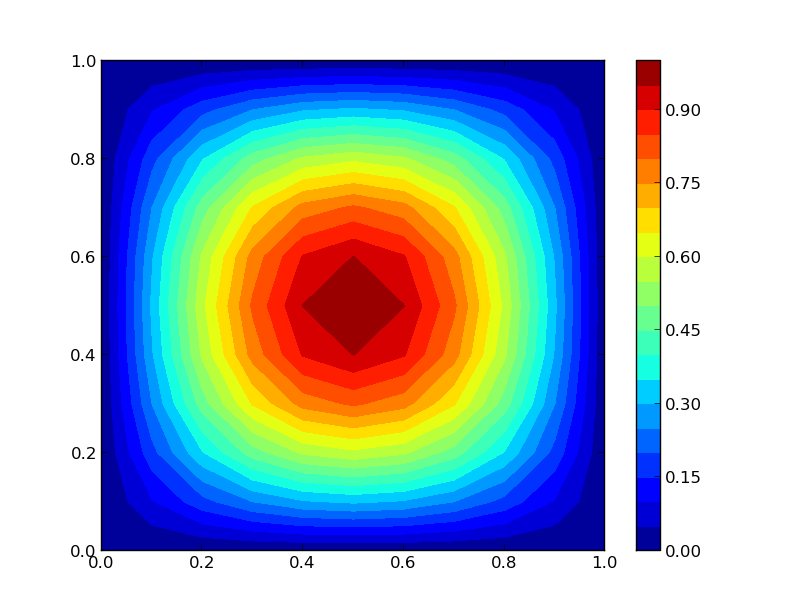
\includegraphics[width=0.7\textwidth]{pix/mesh_example_1}
\end{center}
\end{frame}

\begin{frame}[fragile]
    \frametitle{NumPy}
    \begin{myColorBox}{0.9}{}
\begin{verbatim}
>>> A = np.array( [[1,1], [0,1]] )
>>> B = np.array( [[2,0], [3,4]] )
>>> A*B  # elementwise product
array([[2, 0], 
       [0, 4]])
>>> np.dot(A,B) # matrix product
array([[5, 4],
       [3, 4]])
>>> np.mat(A) * np.mat(B) # matrix product
matrix([[5, 4],
       [3, 4]])
\end{verbatim}
    \end{myColorBox}
There are further functions for array creation, conversions, manipulation, querying, ordering, operations, statistics, basic linear algebra. See NumPy documentation.
\end{frame}

\begin{frame}[fragile]
\frametitle{Numpy}
NumPy subpackages
\begin{itemize}
  \item random: random number generators for various different distributions
  \item linalg: linear algebra tools
  \item fft: discrete Fourier transform
  \item polynomial: efficiently dealing with polynomials
\end{itemize}
\end{frame}

\begin{frame}[fragile]
\frametitle{Numpy}
Example fft:
\begin{myColorBox}{0.9}{}
\begin{verbatim}
>>> sample_rate = 100.0
>>> nsamples = 400
>>> t = np.arange(nsamples) / sample_rate
>>> s = np.cos(2*np.pi*0.5*t) 
+ 0.2*np.sin(2*np.pi*2.5*t+0.1)
>>> S = np.fft.fft(s)
>>> freqs = np.fft.fftfreq(nsamples, 1/samp_rate)
>>> plt.plot(freqs,abs(S))
>>> plt.xlim(-5,5)
>>> plt.show()
\end{verbatim}
\end{myColorBox}
\pause
\begin{center}
      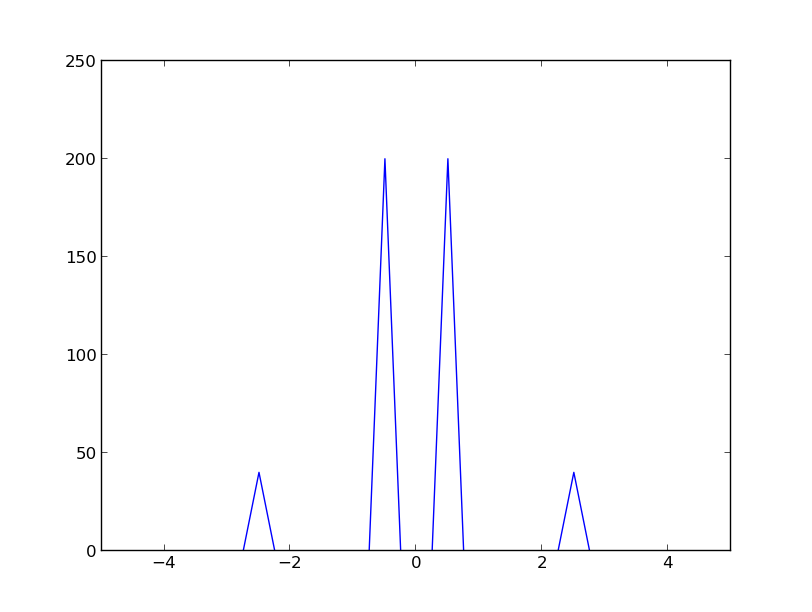
\includegraphics[width=0.5\textwidth]{pix/fft_example_1}
\end{center}
\end{frame}

\begin{frame}
\begin{center}
\Huge{Scipy}
\end{center}
\end{frame}

\begin{frame}
\frametitle{Scipy}
SciPy is a collection of mathematical algorithms and convenience functions built
on the Numpy extension for Python. Scipy subpackages are:
\begin{itemize}
  \item cluster: Clustering algorithms
  \item constants: Physical and mathematical constants
  \item fftpack: Fast Fourier Transform routines
  \item integrate: Integration and ordinary differential equation solvers
  \item interpolate: Interpolation and smoothing splines
  \item io: Input and Output
  \item linalg: Linear algebra
  \item ndimage: N-dimensional image processing
  \item odr: Orthogonal distance regression
  \item optimize: Optimization and root-finding routines
  \item signal: Signal processing
  \item sparse: Sparse matrices and associated routines
  \item spatial: Spatial data structures and algorithms
  \item special: Special functions
  \item stats: Statistical distributions and functions
  \item weave: C/C++ integration               
\end{itemize}
\end{frame}

\begin{frame}[fragile]
\frametitle{Scipy}
Interpolation
\begin{myColorBox}{1.0}{}
\begin{verbatim}
>>> from scipy.interpolate import interp1d
>>> x = np.linspace(0, 10, 10)
>>> y = np.exp(-x/3.0)
>>> f = interp1d(x, y)
>>> f2 = interp1d(x, y, kind='cubic')
>>> xnew = np.linspace(0, 10, 40)
>>> plt.plot(x,y,'o')
>>> plt.plot(xnew,f(xnew),'-',xnew, f2(xnew),'--')
>>> plt.legend(['data', 'linear', 'cubic'], loc='best')
>>> plt.show()
\end{verbatim}
\end{myColorBox}
\pause
\begin{center}
      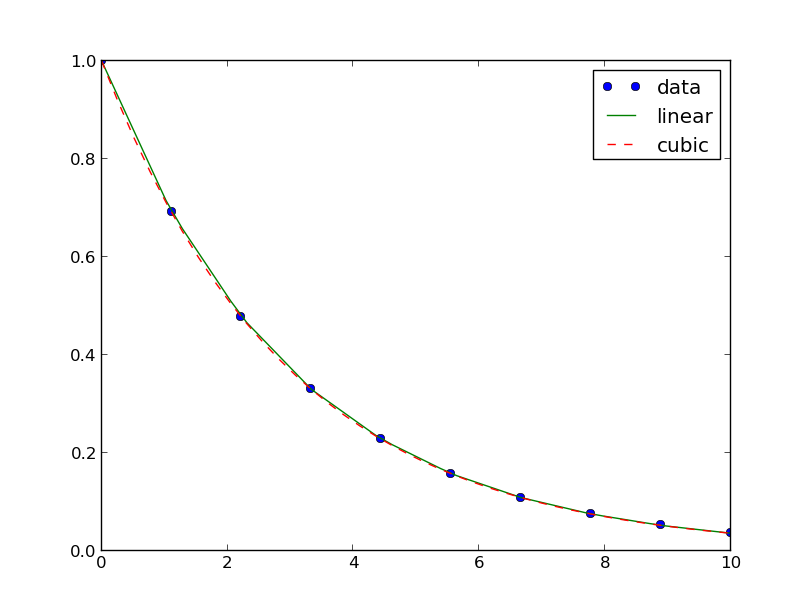
\includegraphics[width=0.5\textwidth]{pix/interpolation_example_1}
\end{center}
\end{frame}

\begin{frame}[fragile]
\frametitle{Scipy}
Least-squares data fitting:
\begin{myColorBox}{1.0}{}
\begin{verbatim}
>>> from scipy import linalg
>>> c1,c2= 5.0,2.0
>>> i = np.arange(1,11)
>>> xi = 0.1*i
>>> yi = c1*np.exp(-xi)+c2*xi
>>> zi = yi + 0.05*np.max(yi)*np.random.randn(len(yi))
# A*c = zi
>>> A = np.array([np.exp(-xi),xi]).T
>>> c,resid,rank,sigma = linalg.lstsq(A,zi)
>>> c
array([ 5.0525305 ,  2.09272423])
>>> resid
0.70716255651624638
\end{verbatim}
\end{myColorBox}
\end{frame}

\begin{frame}[fragile]
\frametitle{Scipy}
\begin{myColorBox}{0.9}{}
\begin{verbatim}
>>> xi2 = np.linspace(0.1,1.0,100)
>>> yi2 = c[0]*np.exp(-xi2) + c[1]*xi2
>>> plt.plot(xi,zi,'x',xi2,yi2)
>>> plt.show()\end{verbatim}
\end{myColorBox}
\pause
\begin{center}
      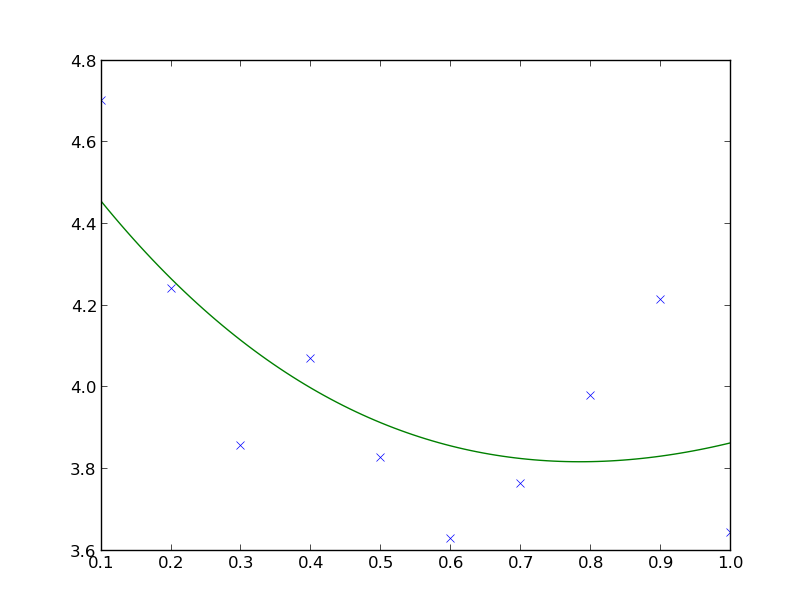
\includegraphics[width=0.5\textwidth]{pix/least_squares_example_1}
\end{center}
\end{frame}

\begin{frame}[fragile]
\frametitle{Scipy}
Loading *.mat files generated by Matlab:
\begin{myColorBox}{1.0}{}
\begin{verbatim}
>> %Matlab
>> mat1 = [1 2 3; 4 5 6; 7 8 9];
>> arr1 = [10 11 12];
>> save test_io.mat mat1 arr1;
\end{verbatim}
\end{myColorBox}
\pause
\begin{myColorBox}{1.0}{}
\begin{verbatim}
>>> from scipy.io import loadmat
>>> a = loadmat('test_io.mat')
>>> a.keys()
['mat1', '__version__', '__header__', 'arr1', ...]
>>>a['mat1']
array([[1, 2, 3],
       [4, 5, 6],
       [7, 8, 9]], dtype=uint8)
>>> a['arr1']
>>> array([[10, 11, 12]], dtype=uint8)
>>> a = loadmat('test_io.mat',squeeze_me=True)
>>> a['arr1']
array([10, 11, 12], dtype=uint8)
\end{verbatim}
\end{myColorBox}
\end{frame}

\begin{frame}[fragile]
\frametitle{Scipy}
\ldots do the reverse:
\begin{myColorBox}{1.0}{}
\begin{verbatim}
>>> from scipy.io import savemat
>>> arr2 = a['arr1']
>>> arr2[0] = 20
>>> savemat('test_io_2.mat',
{'mat1':a['mat1'], 'arr2':arr2},oned_as='row')
\end{verbatim}
\end{myColorBox}
\pause
\begin{myColorBox}{1.0}{}
\begin{verbatim}
>> load test_io_2.mat
>> mat1
mat1 =
    1    2    3
    4    5    6
    7    8    9
>> arr2
arr2 =
   20   11   12
\end{verbatim}
\end{myColorBox}
\end{frame}

\begin{frame}[fragile]
\frametitle{Scipy}
Reading NetCDF files:
\begin{myColorBox}{1.0}{}
\begin{verbatim}
>>> # Reading a GMT grid file
>>> from scipy.io import netcdf
>>> nc = netcdf.netcdf_file('ww3.07121615_GLOBAL05.grd')
>>> nc.variables.keys()
>>> ['y', 'x', 'z']
>>> nc.variables['y'].data
>>> array([-58.5, -58. , -57.5, ..., -31. , -30.5, -30. ])
>>> nc.history
>>> '/usr/local/GMT4.5.7/bin/surface 
-R146.250000/190.000000/-58.500000/-30.000000 
-I0.5 -Gww3.07121615_GLOBAL05.grd 
ww3.07121615_GLOBAL05.xyz'
\end{verbatim}
\end{myColorBox}
\end{frame}

\begin{frame}[fragile]
\frametitle{Documentation}
\begin{itemize}
  \item http://docs.scipy.org/doc/
  \item http://www.scipy.org/Cookbook
  \item http://scipy-central.org/ (code repository)   
\end{itemize}
\end{frame}

\begin{frame}
\begin{center}
\Huge{Exercises}
\end{center}
\end{frame}
